\chapter{Induction}

\newpage

\section{Chauffage par induction}
 
 Un disque métallique de conductivité $\sigma$, d'axe $Oz$ vertical, de rayon $b$ et d'épaisseur $e$ est plongé dans un champ magnétique $\vec{B}$, ayant les caractéristiques suivantes :
\begin{itemize}
\item[-] il est localisé dans un cylindre d'axe vertical $Oz$ et de rayon $a$ ;
\item[-] il est uniforme dans le cylindre précédent et nul à l'extérieur de ce cylindre ;
\item[-] il est dirigé suivant $\vec{e_z}$ ;
\item[-] il varie au cours du temps selon $\vec{B}=B_m\cos(\omega t)\vec{e_z}$.
\end{itemize}

\begin{figure}[h!]
\centering
		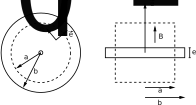
\includegraphics[scale=0.7]{induction1.pdf}
\end{figure}

On admettra par la suite que le champ magnétique induit est négligeable devant le champ magnétique extérieur appliqué. 

\begin{enumerate}

	\item Rappeler l'expression de l'équation de Maxwell-Faraday et justifier l'existence de courants de Foucault dans le cylindre métallique de la forme $\vec{j}=j(r,t)\vec{e_\theta}$.
	
	\item A l'aide de l'équation de Maxwell-Faraday, exprimer $j(r,t)$ en fonction des données du problème.
	
	\item Quelle est l'expression de la puissance dissipée par effet Joule $P_{Joule}$ ? Donner sa valeur moyenne $\langle P_{Joule}\rangle$.
	
	\item Le champ magnétique utilisé a une pulsation de $\omega=1\times10^{5}$rad.s$^{-1}$ et son intensité de l'ordre de $10^{-4}$T. On considère une plaque à induction de rayon $b=10$cm et une casserole dont le fond a le même rayon $a=b=10$cm, une épaisseur $e=3$mm et une conductivité $\sigma=6,0\times10^{7}$S.m$^{-1}$. Déterminer l'ordre de grandeur de la puissance dissipée dans le fond de la casserole.
	
	\item On suppose que le champ magnétique est créé par un solénoïde de 5 cm de longueur ayant un enroulement de $N=100$ spires. En déduire l'intensité $I$ le traversant pour produire le champ magnétique de la question précédente.
	
\end{enumerate}

\newpage

\begin{correction}

\begin{enumerate}

	\item L'équation Faraday s'écrit : $\vv{\mathrm{rot}}\vec{E}=-\partial \vec{B}/\partial t$. Le champ magnétique $\vec{B}$ étant variable, le terme $-\partial \vec{B}/\partial t$ est non nul, et on peut appliquer le théorème d'Ampère (avec $\vec{B}\leftarrow\vec{E}$ et $\mu_0\vec{j}\leftarrow-\partial \vec{B}/\partial t$. Au vu des symétries du problème, on en conclut naturellement que le champ électrique est sous la forme $\vec{E}=E(r,t)\vec{e_\theta}$. Puis par la loi d'Ohm, on en déduit que les courants induits sont de la même forme : $\vec{j}=j(r,t)\vec{e_\theta}$.
	
	\item On calcule tout d'abord le champ électrique à l'aide de la circulation de $\vec{E}$, sur le contour $\Gamma$ choisi comme un cercle de centre $O$ coplanaire au cylindre de rayon $r$, délimitant la surface $\Sigma$ :
	\begin{align*}
		\oint_\Gamma \vec{dl}\cdot\vec{E}=-\oiint_\Sigma\vec{dS}\cdot\frac{\partial \vec{B}}{\partial t}
	\end{align*}
	On est obligé de distinguer les cas $r>a$ et $r<a$ :
	Pour $r<a$ :
	\begin{align*}
		&2\pi r E(r)=\pi r^2B_m \omega \\
		&\Rightarrow E(r)=\frac{rB_m \omega}{2}
	\end{align*}
	Pour $r>a$ :
	\begin{align*}
		&2\pi r E(r)=\pi a^2B_m \omega \\
		&\Rightarrow E(r)=\frac{a^2B_m \omega}{2r}
	\end{align*}	
	La puissance volumique dissipée par effet s'écrit $p_{vol}=\vec{j}\cdot\vec{E}=\gamma E^2(r)$. La puissance totale dissipée sur toute la plaque s'écrit alors :
	\begin{align*}
		P_{vol}&=\iiint_V d\tau p_{vol} \\
		&=\int_0^{2\pi}d\theta\int_0^edz\int_0^ardr\gamma\frac{r^2B_m^2 \omega^2}{4}+\int_0^{2\pi}d\theta\int_0^edz\int_a^brdr\gamma\frac{a^4B_m^2 \omega^2}{4r^2} \\
		&=2\pi e\gamma B_m^2 \omega^2\frac{a^4}{16}+2\pi e \gamma a^4B_m^2\omega^2\frac{1}{4}\ln\left(\frac{b}{a} \right) \\
		&=\frac{1}{2}\pi e\gamma a^4B_m^2 \omega^2\left[\frac{1}{4}+\ln\left(\frac{b}{a} \right) \right] 
	\end{align*}
	
	\item En utilisant la formule précédente, on trouve une puissance de l'ordre de $P=3769$W, ce qui est cohérent avec la puissance maximale des plaques à induction du commerce
	
	\item Le champ créé par un solénoïde est donné par :
	\begin{align*}
		B=\frac{\mu_0 N I}{L}
	\end{align*}
	Pour un champ magnétique de l'ordre de $10^{-4}$T, il faut une intensité $I\simeq0,04$A.
	
\end{enumerate}

\end{correction}